\chapter{Experiments and Results}
\label{c:experiments_and_results}

To verify the claimed properties of FileFarm, we conduct a series of experiments. In this chapter, we will describe our experimental environment first, and then describe settings, process, and results of each experiments.

% Environment
\section{Environment}
\label{s:expenvironment}

In the following experiments, we run FileFarm on 5 physical hosts with following system information:

\begin{itemize}
    \item CPU: Intel(R) Xeon(R) CPU E5-1630 v3 @ 3.70GHz
    \item Memory: 16 GiB DDR4
    \item Network Interface: Ethernet Connection (2) I218-LM (1Gbit/s)
    \item Operating System: Ubuntu Server 18.04.2 LTS
\end{itemize}

 \noindent Each of the 5 physical hosts is assigned with a static IP address, and all of the 5 IP addresses belong to the same subnet with mask 255.255.255.0. Depending on settings of each experiment, a physical host might runs one or multiple instances of FileFarm farmers and clients simultaneously.

\newpage

% exp: LOOKUP Efficiency
\section{Experiment: LOOKUP Efficiency}
\label{s:explookupefficiency}

In FileFarm, each shard is stored on exactly $K$ farmers. Instead of saving location of shards as static records in a centralized database, FileFarm adopts Kademlia's dynamical look up procedures. Thus, the efficiency of these procedures will impact system's I/O performance greatly. According to the sketch of proof in \cite{maymounkov2002kademlia}, LOOKUPs in a Kademlia network will finish in $\lceil log(n) \rceil + c$ steps for some small constant of $c$, where $n$ is network size, i.e., number of nodes in the network. We want to verify that this property also holds in FileFarm.

In this experiment, we start $m$ farmers on each physical host; thus there are $n = 5 \times m$ farmers in total. After all farmers are bootstrapped, we make each farmer LOOKUP 10 random targets and report the number of hops needed to locate the $K$ closest farmers around the target. Then we collect and compute mean of hops needed. The whole process is repeated for $m=1,2,5,10,20,50$ and $K=1,2,3,4,5$.

\begin{figure}[hbt]
\centering
  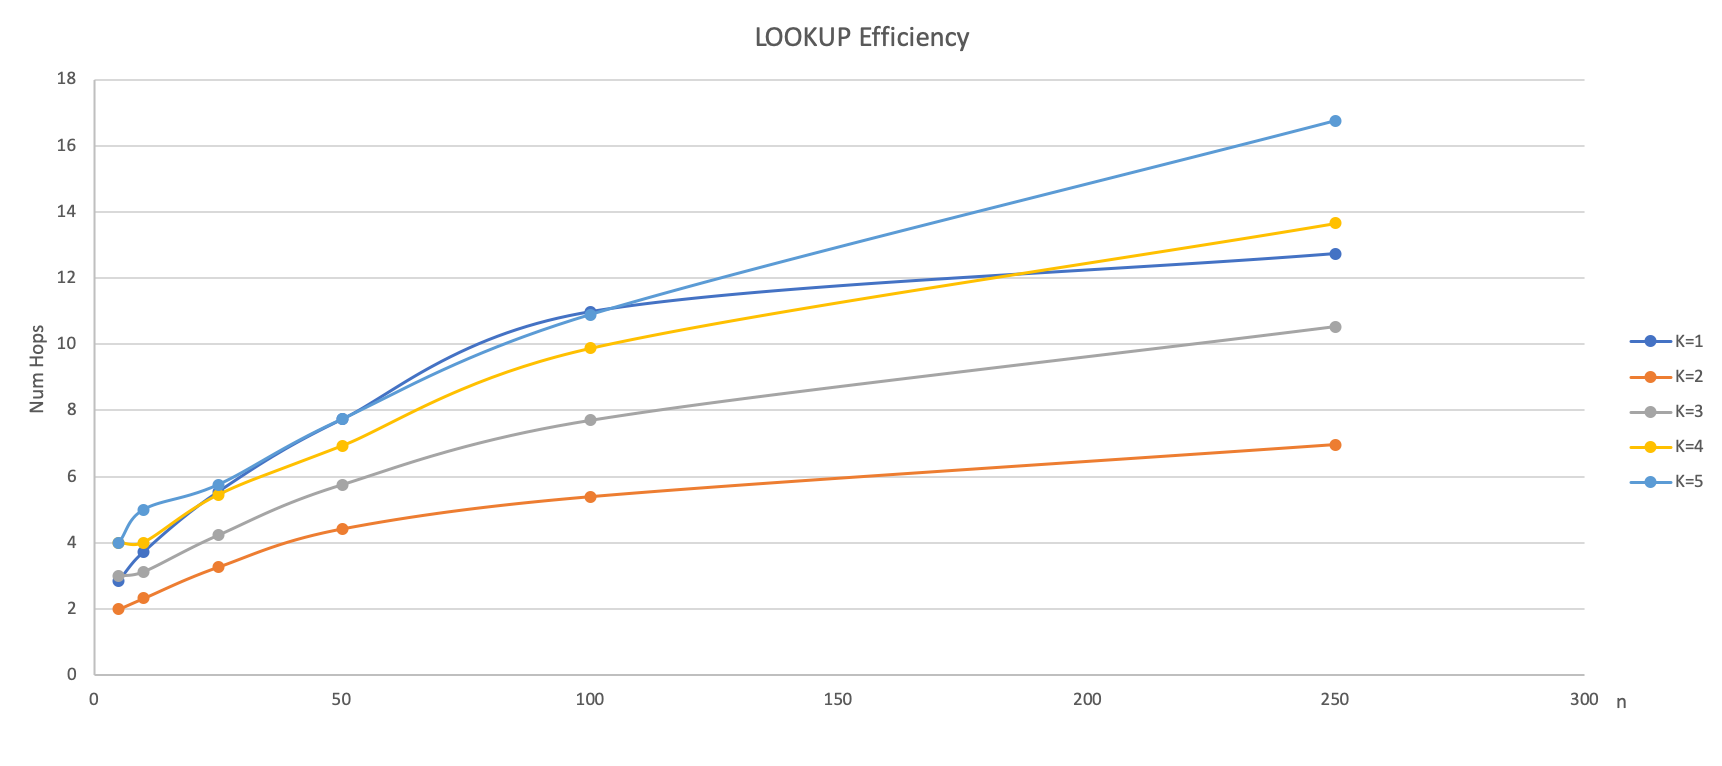
\includegraphics[width=14cm]{charts/chart_lookup_efficiency.png}
  \caption{Number of LOOKUP steps (hops) with respect to $K$ and network size}
  \label{fig:lookupefficiency}
\end{figure}

From Figure \ref{fig:lookupefficiency}, we can observe that number of LOOKUP steps grows with number of farmers, following a logarithm-like curve. With number of farmers growing from 100 to 200, it only takes around 2 more steps to locate all $K$ closest farmers, which makes FileFarm network scalable. However, it can also be observed that a larger setting of $K$ requires more steps for LOOKUP procedure to finish, which is intuitive, considering the fact that LOOKUP finds all of the $K$ closest farmers but not one or some of them.


% exp: VALUE_LOOKUP Efficiency
\section{Experiment: VALUE\_LOOKUP Efficiency}
\label{s:expvaluelookupefficiency}

Just like performing LOOKUP before uploading a shard, farmers perform VALUE\_LOOKUP before downloading a shard. Different from LOOKUP, the VALUE\_LOOKUP procedure finishes immediately when the target value is found. Thus, VALUE\_LOOKUP procedure only needs to reach any one of the $K$ closest farmers instead of finding all of them. According to Cai's analysis\cite{cai2013probabilistic}, it takes no more than $(1+O(1))\frac{log(n)}{H_{K}}$ steps for any node in a Kademlia network to locate any other node, where $H_K = \sum_{i=1}^{K} 1/i$. This upper bound also stands for VALUE\_LOOKUP, considering the fact that VALUE\_LOOKUP for the target key converges along the same path as LOOKUP for the closest farmer, due to $unidirectionality$ of XOR distance metrics. In this experiment, we want to verify this property on FileFarm and compare the result with \ref{s:explookupefficiency}.

In this experiment, we start $m$ farmers on each physical host; thus there are $n = 5 \times m$ farmers in total. After all farmers are bootstrapped, we starts 1 client on each physical hosts and make them upload 100 random files in total. Then we make each client send 200 file download requests randomly and let farmers report the number of hops needed for each VALUE\_LOOKUP. We collect and compute mean of hops needed. The whole process is repeated for $m=1,2,5,10,20,50$ and $K=1,2,3,4,5$.

\begin{figure}[hbt]
\centering
  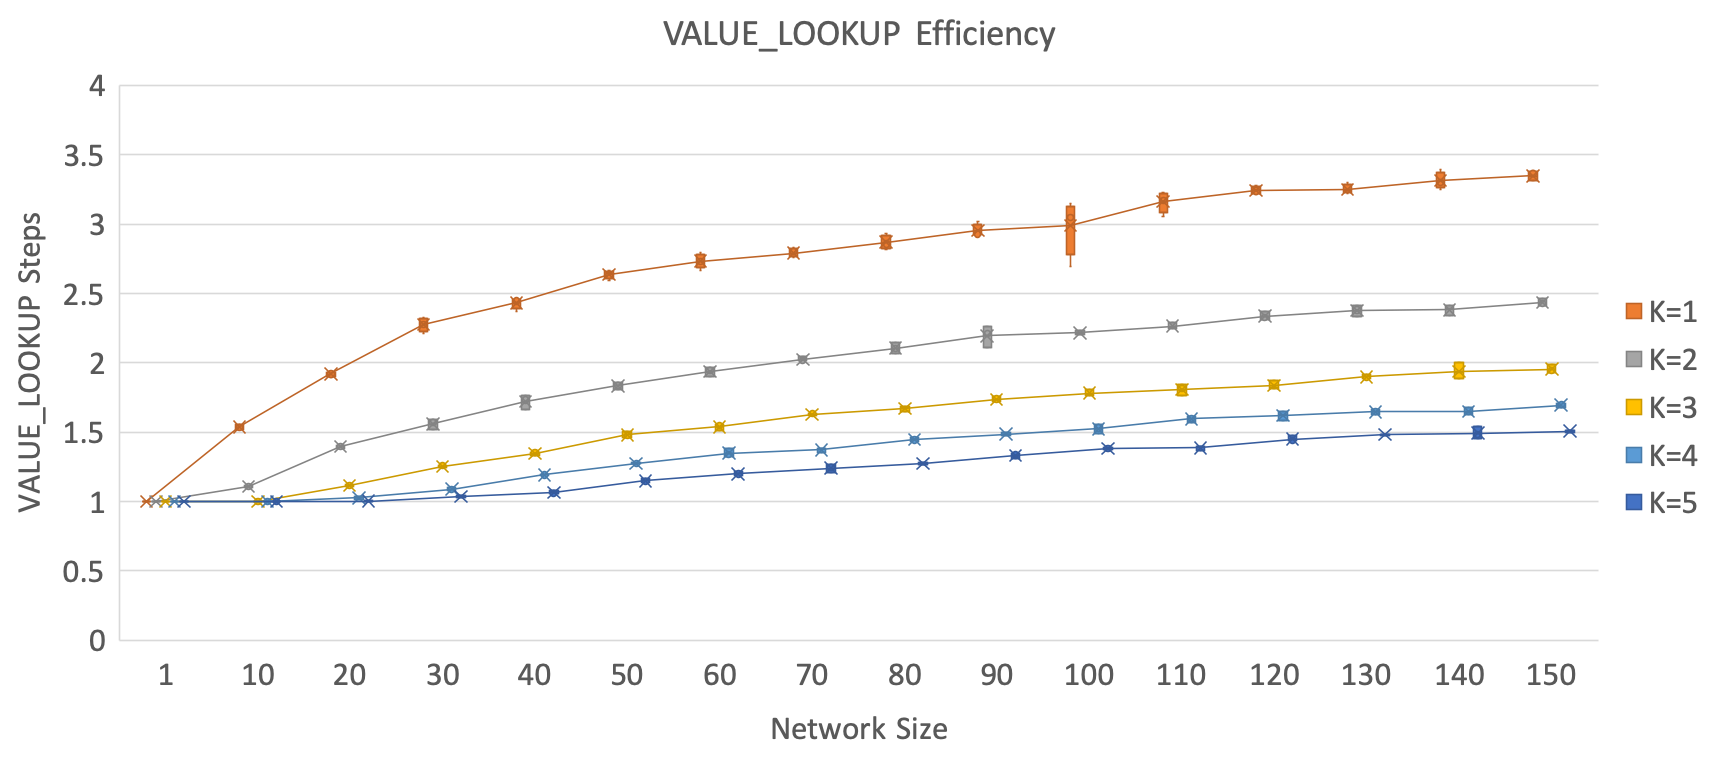
\includegraphics[width=14cm]{charts/chart_value_lookup_efficiency.png}
  \caption{Number of VALUE\_LOOKUP hops with respect to $K$ and network size}
  \label{fig:valuelookupefficiency}
\end{figure}

From figure \ref{fig:valuelookupefficiency}, we can observe that VALUE\_LOOKUP also follows a logarithm curve, but the number of hops needed is far less than that needed by LOOKUP shown in \ref{fig:lookupefficiency}. In a FileFarm network of 100 farmers, it only takes less than 3 hops to find a shard. Besides, as $K$ increases, number of hops decreases roughly with a factor $H_{K}$ depicted by Cai\cite{cai2013probabilistic}. Putting this result with \ref{s:explookupefficiency}, we can conclude that a larger choice of $K$ results in more uploading overhead, while improves download performance.

% exp: Retrievability
\section{Experiment: Retrievability}
\label{s:expretrievability}

% exp: Throughput
\section{Experiment: Throughput}
\label{s:expthroughput}

In this experiment, we want to test FileFarm's I/O performance under different file size and sharding schemes. As described in figure \ref{fig:uploadflow} and figure \ref{fig:downloadflow}, the upload process of FileFarm involves slicing, encryption, IDA computation, LOOKUP, ... while the download process involves VALUE\_LOOKUP, IDA computation, decryption, combining... Some operations can be done in parallel, while others cannot. To analyze performance of such complicated flows, we run experiments and measure the elapsed time.

As for the experimental procedure, we runs 5 farmers and 25 clients in total. Each farmer is assumed to have a 10 MB/s upload bandwidth. Once all farmers and clients are bootstrapped, we let clients start random upload and download files of size $S$ with a sharding scheme which generates $p$ shards in total. While uploading and downloading, we let clients report time consumption for each operations until 100 upload and 100 download reports have been collected. We collect these reports and compute mean of upload/download throughput. The whole process is repeated for $S=1,4,16,64,256,1024$ and $p=1,2,4,8,16,32$.

\begin{figure}[hbt]
\centering
  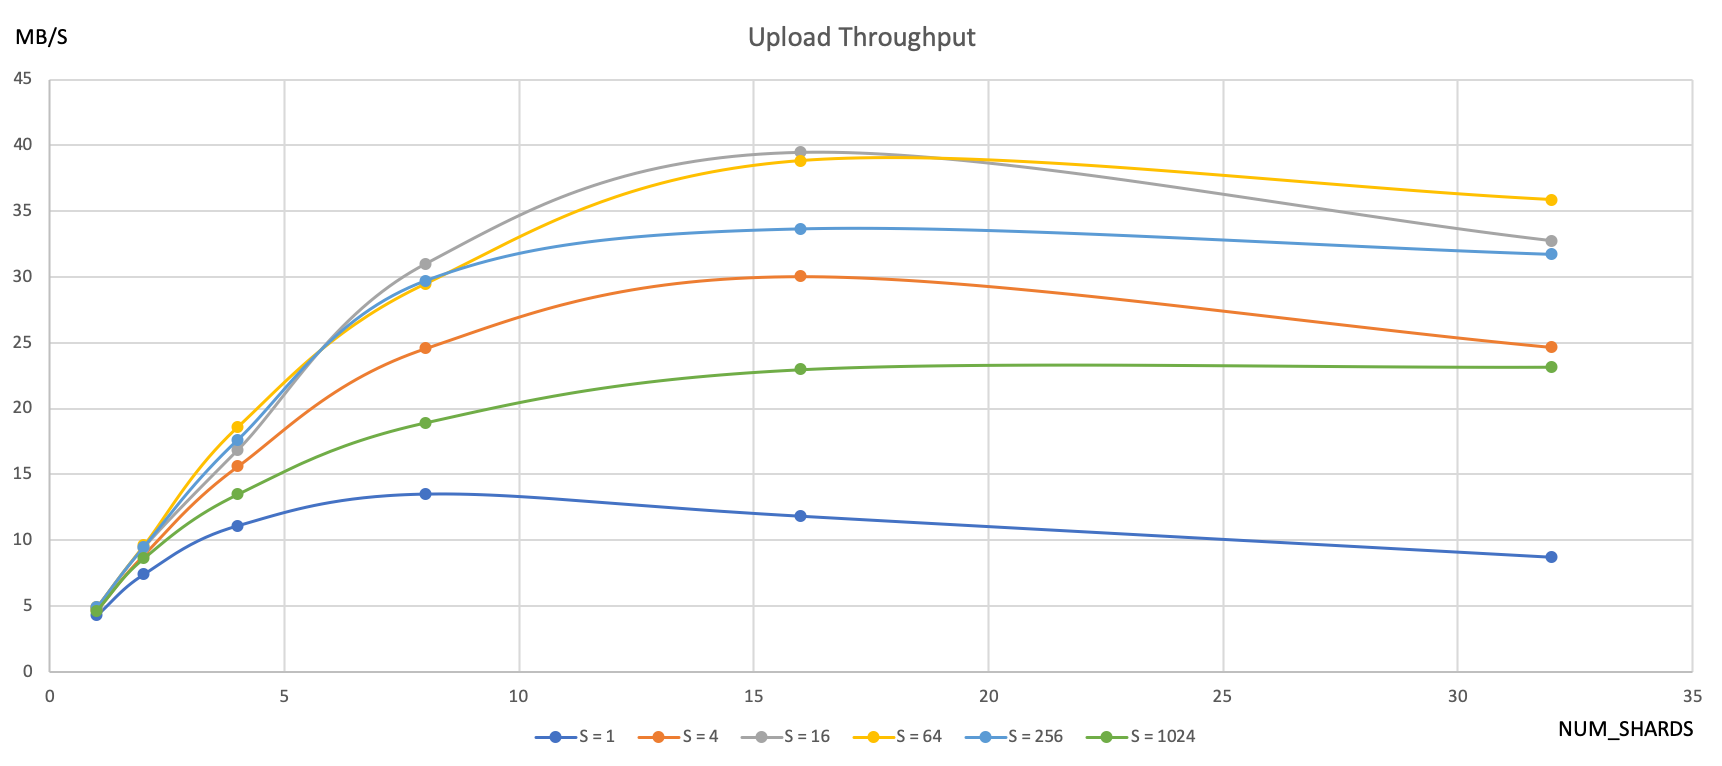
\includegraphics[width=14cm]{charts/chart_upload_throughput.png}
  \caption{Upload throughput with respect to file size and number of shards}
  \label{fig:uploadthroughput}
\end{figure}

\begin{figure}[hbt]
\centering
  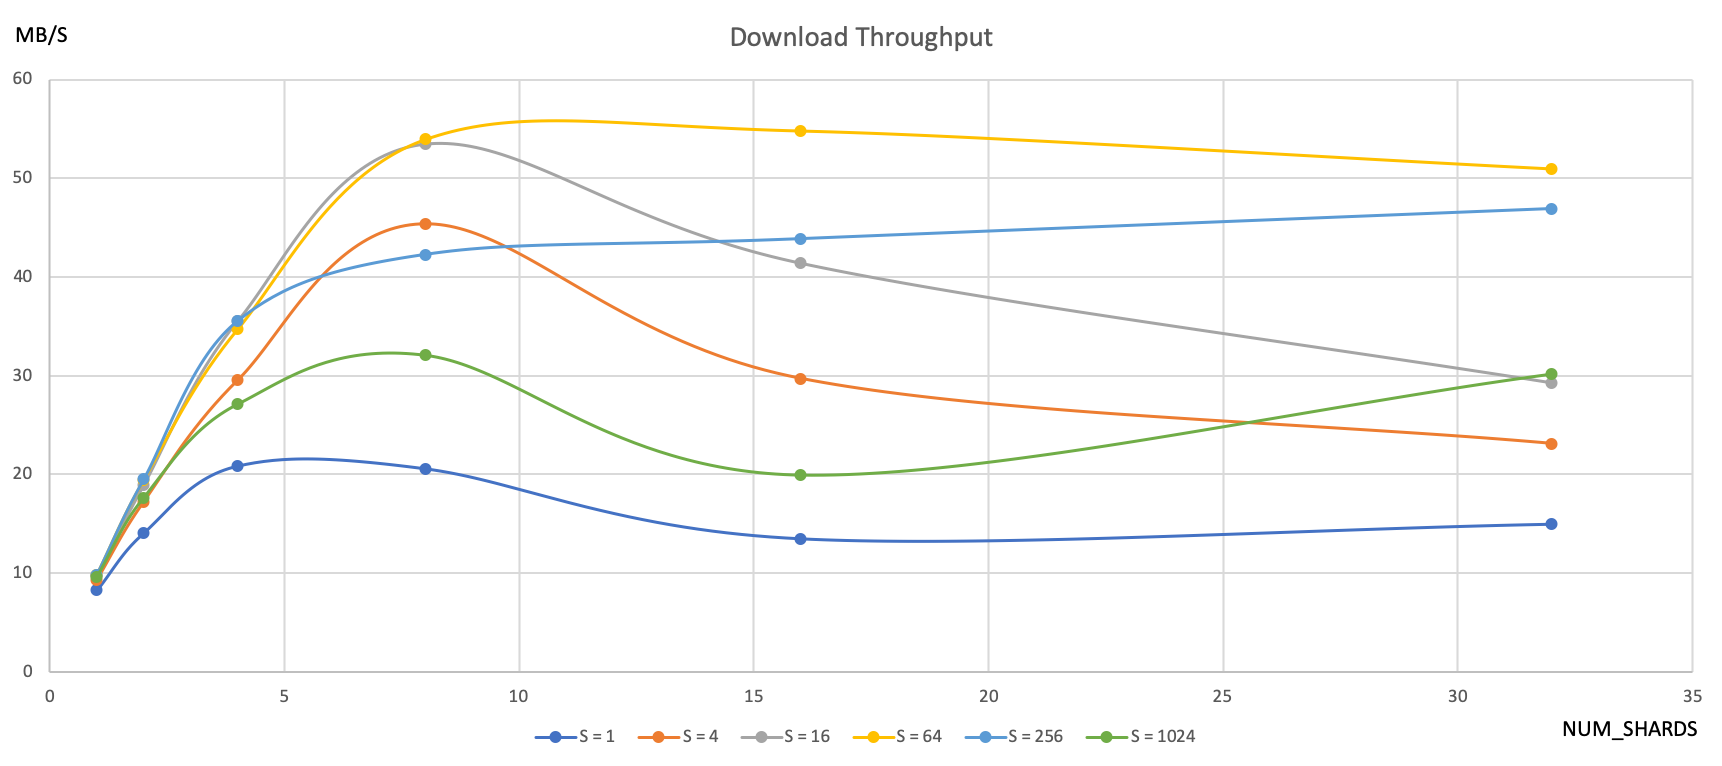
\includegraphics[width=14cm]{charts/chart_download_throughput.png}
  \caption{Download throughput with respect to file size and number of shards}
  \label{fig:downloadthroughput}
\end{figure}

From the result shown in figure \ref{fig:uploadthroughput}, we observe that uploading throughput grows when number of shards increases. This trends achieve peak value when number of shards = 16. After that, the curve goes down. With a file of size 64 MB, a sharding schema in which $p=16$ brings a best performance of around 39 MB/s.

Due to the procedural differences, the chart of download throughput, figure \ref{fig:downloadthroughput} seems different from that of upload throughput. First, the curves achieve peak value when number of shards is around 8. Second, download throughput is generally higher than upload throughput. This is because of the fact that download only involves retrieval of 1 copy of the target shard instead of $K$. Considering figure \ref{fig:uploadthroughput} and figure \ref{fig:downloadthroughput} collectively, we can conclude that under this scenario, choices of \#shards = 8 or 16 brings the best I/O performance in general.

% exp: Cost Efficiency
\section{Experiment: Cost Efficiency}
\label{s:expcostefficiency}